\clearpage
\section{镜中的第二面镜子}

打开“实时效果”中的 SSR 和“屏幕外反射”，再调“镜面反射次数”。下面的小场景只放两面镜子、灯牌、地面与墙。方向光照亮地面，天空反射和间接光都关闭。左图限制一次反射，只能查到第二面镜子。右图允许第二段射线继续向灯牌查找。灯牌在相机画面之外，它的颜色由网格材质给出。

\begin{center}
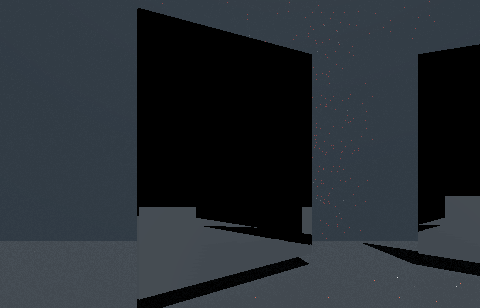
\includegraphics[width=.48\linewidth]{../../../output/validation/mirror-bounces/one.png}\hfill
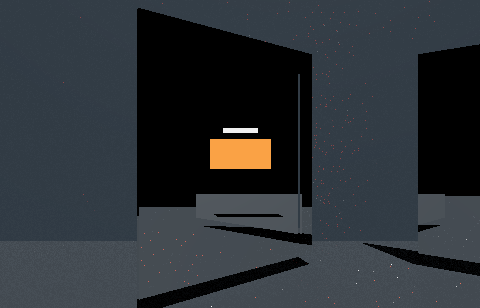
\includegraphics[width=.48\linewidth]{../../../output/validation/mirror-bounces/two.png}\\
{\small 同一台相机，第 8 帧的 Vulkan 面板。中间的白色短灯条可以用来辨认色块的上下方向。}
\end{center}

为了弄清橙色来自哪一路光，在 RenderDoc 中分别读取反射计算前后的线性 RGB。取图像正中央 $5\times5$ 个像素的平均值，单位沿用场景的线性光照值。灯牌材质的发光色设为 $(3.20,0.24,0.06)$。允许两次反射后，中央增加的正是这个值。只给第二面镜子换上少反红光的材质，传回来的红色降为 0.805。最后将挡板放在第二面镜子与灯牌之间，灯牌消失。

{\smalltable\noindent\begin{tabularx}{\linewidth}{@{}Xrrr@{}}\toprule
镜子和灯牌 & 红 & 绿 & 蓝\\\midrule
白色镜子，一次反射 & 0.000 & 0.000 & 0.000\\
白色镜子，两次反射 & 3.200 & 0.240 & 0.060\\
灯牌改为蓝光 & 0.080 & 0.400 & 2.400\\
第二面镜子的金属底色改为 $(0.25,1,0.5)$ & 0.805 & 0.240 & 0.030\\
保持橙色灯牌，加入挡板 & 0.000 & 0.000 & 0.000\\\bottomrule
\end{tabularx}\par}

把同一块绿灯牌放在第三或第四面镜子之后，分别把次数限制在离灯牌还差一段的位置，再增加一次反射。两次实验中，中央都从接近零变为 $(0.180,2.100,0.570)$，与绿灯牌的材质相符。

在 RTX 5070 Ti Laptop GPU 上使用 Debug 构建，面板为 $480\times308$。一次与两次反射的计算事件均为 132，分别位于各自的帧文件。RenderDoc 1.47 预热一次后回放 11 次，GPU 时间的中位数为 0.132 和 0.234\,ms。这两数衡量反射这一道计算；此场景的三角形数量很少，复杂关卡的成本要另测。

“反射距离”约束每一段射线能查找的距离。第一段也检查本帧屏幕中的表面，可找到镜头看得见的运动角色；后续各段从场景保存的静态三角形中取交点。粗糙表面每段只取一个方向，图中光滑的金属镜可以得到稳定轮廓。渲染入口在 \path{Redflag/src/Redflag/Renderer/ScreenSpace/Shaders/StochasticSSR.comp} 的 \texttt{reflectScenePath}。从仓库根目录执行 \texttt{python tests/check\_mirror\_bounces.py} 可重建场景、截帧并核对这些颜色。每份原始帧的校验值、事件和计时记录在 \path{output/validation/mirror-bounces/}。

\clearpage
\section{维修站开场的倒影}

从工作间的小镜子回到维修站，画面大半被砂石路和漆面设备占据。这里也打开两次反射，远没有两面光滑金属镜里的灯牌那么显眼。左图是这一版维修站固定主相机的 Vulkan 画面。右图用白色标出把次数从一改成二以后，面板中红、绿、蓝至少有一个通道变化超过 $2/255$ 的像素。这个数相当于八位图像里相邻的两级颜色，用来画差别的位置。

\begin{center}
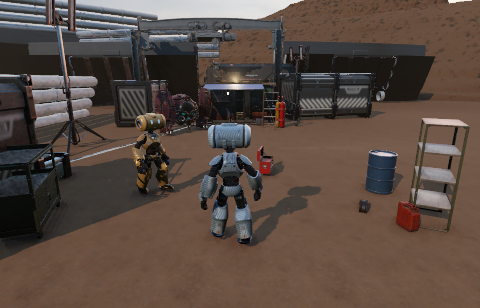
\includegraphics[width=.48\linewidth]{../../../output/validation/mirror-bounces/yard-2.png}\hfill
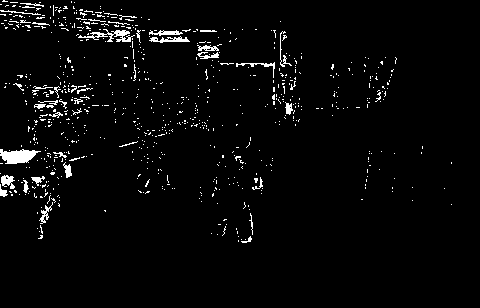
\includegraphics[width=.48\linewidth]{../../../output/validation/mirror-bounces/yard-change.png}\\
{\small 维修站初始机位及同机位的逐像素差别。角色姿态固定在动画的第零秒。}
\end{center}

RenderDoc 1.47 回放第 8 帧。在 $480\times308$ 个像素上，两份截帧的材质以及送入反射计算的颜色逐个相同。显示图中共有 4,608 个像素超过上面的门槛，约占 3.12\%。这一机位可以看到设备和角色上的局部差别，要辨认镜中灯牌的完整形状，仍可打开上一页的两面镜子实验。

RTX 5070 Ti Laptop GPU 对这一道计算预热一次，再各回放 11 次，耗时的中位数从 0.847 升到 1.590\,ms。取样用 Debug 构建；这里计的是反射事件自身，后面还会单独降噪。之后关卡若改了机位或金属材质，受影响的屏幕面积也会改变。这一版的场景指纹、截帧、计时和颜色差记录在 \path{output/validation/mirror-bounces/yard.json}。
